%%%%%%%%%%%%%%%%%%%%%%%%%%%%%%%%%%%%%%%%%%%%%%%
%%%     Declarations (skip to Begin Document, line 88, for parts you fill in)
%%%%%%%%%%%%%%%%%%%%%%%%%%%%%%%%%%%%%%%%%%%%%%%

\documentclass[10pt]{article}

\usepackage{geometry}  % Lots of layout options.  See http://en.wikibooks.org/wiki/LaTeX/Page_Layout
\geometry{letterpaper}  % ... or a4paper or a5paper or ... 
\usepackage{fullpage}  % somewhat standardized smaller margins (around an inch)
\usepackage{setspace}  % control line spacing in latex documents
\usepackage[parfill]{parskip}  % Activate to begin paragraphs with an empty line rather than an indent

\usepackage{amsmath,amssymb}  % latex math
\usepackage{empheq} % http://www.ctan.org/pkg/empheq
\usepackage{bm,upgreek}  % allows you to write bold greek letters (upper & lower case)

\usepackage{soul}  % for hl and friends

% for typsetting algorithm pseudocode see http://en.wikibooks.org/wiki/LaTeX/Algorithms_and_Pseudocode
\usepackage{algorithmic,algorithm}  

\usepackage{graphicx}  % inclusion of graphics; see: http://en.wikibooks.org/wiki/LaTeX/Importing_Graphics
% allow easy inclusion of .tif, .png graphics
\DeclareGraphicsRule{.tif}{png}{.png}{`convert #1 `dirname #1`/`basename #1 .tif`.png}

\usepackage{subfigure}  % allows subfigures in figure

\usepackage{xspace}
\newcommand{\latex}{\LaTeX\xspace}

\usepackage{color}  % http://en.wikibooks.org/wiki/LaTeX/Colors

\long\def\ans#1{{\color{blue}{\em #1}}}
\long\def\ansnem#1{{\color{blue}#1}}
\long\def\boldred#1{{\color{red}{\bf #1}}}
\long\def\boldred#1{\textcolor{red}{\bf #1}}
\long\def\boldblue#1{\textcolor{blue}{\bf #1}}

% Useful package for syntax highlighting of specific code (such as python) -- see below
\usepackage{listings}  % http://en.wikibooks.org/wiki/LaTeX/Packages/Listings
\usepackage{textcomp}

%%% The following lines set up using the listings package
\renewcommand{\lstlistlistingname}{Code Listings}
\renewcommand{\lstlistingname}{Code Listing}

%%% Specific for python listings
\definecolor{gray}{gray}{0.5}
\definecolor{green}{rgb}{0,0.5,0}

\lstnewenvironment{python}[1][]{
\lstset{
language=python,
basicstyle=\footnotesize,  % could also use this -- a little larger \ttfamily\small\setstretch{1},
stringstyle=\color{red},
showstringspaces=false,
alsoletter={1234567890},
otherkeywords={\ , \}, \{},
keywordstyle=\color{blue},
emph={access,and,break,class,continue,def,del,elif ,else,%
except,exec,finally,for,from,global,if,import,in,i s,%
lambda,not,or,pass,print,raise,return,try,while},
emphstyle=\color{black}\bfseries,
emph={[2]True, False, None, self},
emphstyle=[2]\color{green},
emph={[3]from, import, as},
emphstyle=[3]\color{blue},
upquote=true,
morecomment=[s]{"""}{"""},
commentstyle=\color{gray}\slshape,
emph={[4]1, 2, 3, 4, 5, 6, 7, 8, 9, 0},
emphstyle=[4]\color{blue},
literate=*{:}{{\textcolor{blue}:}}{1}%
{=}{{\textcolor{blue}=}}{1}%
{-}{{\textcolor{blue}-}}{1}%
{+}{{\textcolor{blue}+}}{1}%
{*}{{\textcolor{blue}*}}{1}%
{!}{{\textcolor{blue}!}}{1}%
{(}{{\textcolor{blue}(}}{1}%
{)}{{\textcolor{blue})}}{1}%
{[}{{\textcolor{blue}[}}{1}%
{]}{{\textcolor{blue}]}}{1}%
{<}{{\textcolor{blue}<}}{1}%
{>}{{\textcolor{blue}>}}{1},%
%framexleftmargin=1mm, framextopmargin=1mm, frame=shadowbox, rulesepcolor=\color{blue},#1
framexleftmargin=1mm, framextopmargin=1mm, frame=single,#1
}}{}
%%% End python code listing definitions

% \DeclareMathOperator{\diag}{\texttt diag}
\DeclareMathOperator{\diag}{\mathrm{diag}}
\DeclareMathOperator{\cov}{\texttt cov}
% \DeclareMathOperator{\cov}{\mathrm{cov}}

%% hilite
\newcommand{\hilite}[1]{\colorbox{yellow}{#1}}
\long\def\todo#1{\hilite{{\bf TODO:} {\em #1}}}

%%%%%%%%%%%%%%%%%%%%%%%%%%%%%%%%%%%%%%%%%%%%%%%
%%%     Begin Document
%%%%%%%%%%%%%%%%%%%%%%%%%%%%%%%%%%%%%%%%%%%%%%%

\begin{document}

\begin{center}
    {\Large {\bf ISTA 421/521 -- Homework 3}} \\
    \boldred{Due: Friday, October 8, 5pm} \\
    24 pts total for Undergrads, 30 pts total for Grads
    
\end{center}

\begin{flushright}
STUDENT NAME %% Fill in your name here

Undergraduate / Graduate %% select which you are!
\end{flushright}

\vspace{1cm}
{\Large {\bf Instructions}}

In this assignment you are required to modify/write 4 scripts in python.  Details of what this will involve are specified in exercises 1, 2, 5 and 6, below.

Included in the homework 3 release are following files in {\tt code}:
\begin{itemize}
\item{\tt poisson.py} - This script will be used in Exercise 1.
\item{\tt random\_generator.py} - This script implements a class, {\tt RNG}, that will simulate a random number generator, but where the random numbers are read from file. This is an attempt to make it so that all random number draws will be uniform across platforms. This will be used in Exercise 2.
\item {\tt approx\_expected\_value.py} - This script includes a demonstration of how to approximate an expected value through sampling.  You will modify this code and submit your solution for Exercise 2.
\item {\tt predictive\_variance.py} - This script contains code relevant to exercises 5 and 6. You will need to fill in two functions (as described in Exercise 5) as well as {\tt exercise\_6}
\item {\tt gauss\_surf.py} - This is provided for fun -- it is not required for any exercise here. It generates a 2d multivariate Gaussian and plots it as both a contour and surface plot. This provides an example of how to code making use of numpy array-computation; in particular, look at how the ``mesh'' of points in 2-d surface is computed simultaneously on lines 84-95 (see comments).
\item {\tt w\_variation\_demo.py} - This script is also provided for fun and is not required for the assignment. (It also provides more example python code!)  This implements the simulated experiment demonstrating the theoretical and empirical bias in the estimate, $\widehat{\sigma^2}$, of the model variance, $\sigma^2$, as a function of the sample size used for estimation.
\end{itemize}

All exercises except exercise 1 require that you provide some ``written'' answer (in some cases also figures), so you will also submit a .pdf of your written answers.  You can use \latex or any other system (including handwritten; plots, of course, must be program-generated) as long as the final version is in PDF. 

As with the previous homework, the final submitted PDF written answers must be named {\tt hw3-answers.pdf}.

NOTE: Exercises 3 and 7 are required for Graduate students only; Undergraduates may complete them for extra credit equal to the point value.

As in previous homework, pytest ``unit tests'' are provided to help guide your progress.

You may work with others in the course on the homework. However, if you do, you. {\bf must} list he names of everyone you worked with, along with which problems you collaborated. Your final submissions of code and written answers {\bf MUST ALL BE IN YOUR OWN CODE FORMULATION AND WORDS}; you cannot submit copies of the same work -- doing so will be considered cheating.

(FCML refers to the course text: Rogers and Girolami (2016), {\em A First Course in Machine Learning, Second Edition}.  For general notes on using \latex to typeset math, see:\\ {\tt http://en.wikibooks.org/wiki/LaTeX/Mathematics})
\vspace{.5cm}

%%%%%%%%%%%%%%%%
%%%     Exercises
%%%%%%%%%%%%%%%%

% \newpage
\begin{itemize}

%%%     Exercise 1
\item[1.] [3 points]
Adapted from {\bf Exercise 2.3} of FCML:

Let $Y$ be a random variable that can take any non-negative integer value.  The likelihood of these outcomes is given by the Poisson pmf (probability mass function):
\begin{eqnarray}
P(y) = {\lambda^y\over y!} e^{-\lambda}
\end{eqnarray}
By using the fact that for a discrete random variable the pmf gives the probabilities of the individual events occurring and the probabilities are additive, fill in the two functions in {\tt poisson.py} as follows:
\begin{enumerate}
\item[(a)] In {\tt calculate\_posson\_pmf\_a} compute the probability that $Y \geq 3$ and $Y \leq 7$ for $\lambda = 5$, i.e., $P(3 \leq Y \leq 7)$, and assign that to the return value {\tt probability}.
\item[(b)] In {\tt calculate\_posson\_pmf\_b}, using the fact that one outcome has to happen, compute the {\tt probability} that $Y < 3$ or $Y > 7$ (again, for $\lambda = 5$).
\end{enumerate}
You are only allowed to use the python {\tt math} package; no other packages are allowed.

There is no need for a written answer to this exercise, only your code submission.

% {\bf Solution.} %$<$Solution goes here$>$


%%%     Exercise 2
\item[2.] [4 points]
Adapted from {\bf Exercise 2.4} of FCML:

Let $X$ be a random variable with uniform density, $p(x) = \mathcal{U}(a,b)$.

Work out analytically $\mathbf{E}_{p(x)} \left\{ 35 + 3x - 0.5x^3 + 0.05x^4 \right\}$ for $a=-4$, $b=10$ (show the steps).  

The script {\tt approx\_expected\_value.py} includes a function that demonstrates how you can use uniform random samples to approximate an expectation, as described in Section 2.5.1 of FCML.  The script estimates the expectation of the function $y^2$ when $Y \sim \mathcal{U}(0,1)$ (that is, $Y$ is uniformly distributed between $0$ and $1$).  This script generates a plot of how the estimation improves as larger samples are considered, up to 1000 samples.

Fill in the function {\tt exercise\_2} in {\tt approx\_expected\_value.py} to compute a sample-based approximation to the expectation of the function $35 + 3x - 0.5x^3 + 0.05x^4$ when $X \sim \mathcal{U}(-4,10)$ and observe how the approximation improves with the number of samples drawn.  In your written answer, include the generated plot {\tt ex2\_fn\_approx.png} showing the evolution of the approximation, relative to the true value, over $10,000$ samples. Include a description of the trend you see in the plot.

{\bf Solution.}

%%% For latex users: code to insert figure, and update the caption to describe the figure!
%\begin{figure}[h!]
%\begin{center}
%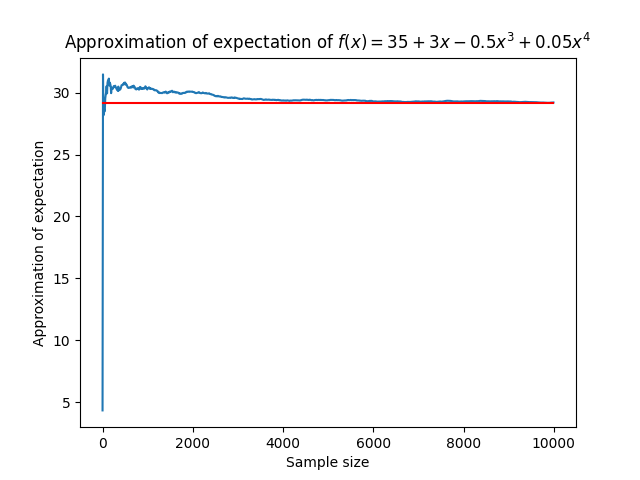
\includegraphics[width=10cm]{figures/ex2_fn_approx.png}
%\caption{Your Caption Here.\label{fig:approx}}
%\end{center}
%\end{figure}


%%%     Exercise 3
\item[3.] [2 points; \boldred{Required only for Graduates}]
Adapted from {\bf Exercise 2.6} of FCMA:

Assume that $p(\mathbf{w})$ is the Gaussian pdf for a $D$-dimensional vector $\mathbf{w}$ given in
\begin{eqnarray}
p(\mathbf{w}) = \frac{1}{(2 \pi)^{D/2} | \mathbf{\Sigma} |^{1/2}} \exp \left\{ -\frac{1}{2} (\mathbf{w} - \mathbf{\mu})^\top \mathbf{\Sigma}^{-1} (\mathbf{w} - \mathbf{\mu}) \right\} . \label{eqn:multnormal}
\end{eqnarray}

Suppose we use a diagonal covariance matrix with different elements on the diagonal, i.e.,
\begin{eqnarray*}
\mathbf{\Sigma} = 
\begin{bmatrix}
\sigma_1^2 & 0 & \cdots & 0 \\
0 & \sigma_2^2 & \cdots & 0 \\
\vdots & \vdots & \ddots & \vdots \\
0 & 0 & \cdots & \sigma_D^2
\end{bmatrix}
\end{eqnarray*}

Does this assume independence of the $D$ elements of $\mathbf{w}$?  If so, show how by expanding the vector notation of Eqn.~\ref{eqn:multnormal} and re-arranging.  You will need to be aware that the determinant of a matrix that only has entries on the diagonal is the product of the diagonal values and that the inverse of the same matrix is constructed by simply inverting each element on the diagonal.  (Hint, a product of exponentials can be expressed as an exponential of a sum.  Also, just a reminder that $\exp\{x\}$ is $e^x$.)

{\bf Solution.}



%%%     Exercise 4
\item[4.] [4 points]
Adapted from {\bf Exercise 2.9} of FCML:

Assume that a dataset of $N$ binary values, $x_1, ..., x_N$, was sampled from a Bernoulli distribution, and each sample $x_i$ is independent of any other sample.  Explain why this is {\em not} a Binomial distribution.  Derive the maximum likelihood estimate for the Bernoulli parameter of this distribution.

{\bf Solution.} 



%%%     Exercise 5
\item[5.] [8 points]
Adapted from {\bf Exercise 2.12} of FCML:

Familiarize yourself with the provided script {\tt predictive\_variance.py}.  
It is mostly implemented, but you will have to fill in the details for two functions: 
\begin{itemize}
\item {\tt calculate\_prediction\_variance}, which calculates the {\em variance} for a prediction at $x_{\mathrm{new}}$ given the design matrix, $\mathbf{X}$, the estimated parameters, $\mathbf{\hat{w}}$, and target responses, $\mathbf{t}$.
\item {\tt calculate\_cov\_w}, which calculates the estimated covariance of $\mathbf{\hat{w}}$ given the design matrix, $\mathbf{X}$, the estimated parameters, $\mathbf{\hat{w}}$, and target responses, $\mathbf{t}$.
\end{itemize}
Once implemented, then you can run the script.

When you run the script, it will generate a dataset based on a function (implemented in {\tt true\_function}) and then remove all values for which $-1 \leq x \leq 1$.  Three groups of plots will be generated:
\begin{enumerate}
\item[(a)] First is a plot of the data (this will be generated by Part 5a of the script).  
\item[(b)] Next, the script will plot the error bar plots for predictions of values for model orders 1, 3, 5 and 9 (this will be generated by Part 5b).  
\item[(c)] Finally, in Part 5c, the script samples model parameters $\mathbf{\hat{w}}$ from the covariance $\cov(\mathbf{\hat{w}})$ and plots the resulting functions (again, for model orders 1, 3, 5 and 9).
\end{enumerate}

In total, you will plot 9 figures. You must include the plots in your written submission and do the following: Include a caption for each figure that qualitatively describes what the figure shows; contrast the figures within group (b) with each other. Do the same for group (c).  Also, clearly explain what effect removing the points $-1 \leq x \leq 1$ has done in contrast to if they were left in.

(NOTE: the script {\tt predictive\_variance} also contains elements for Exercise 6 (namely, the function {\tt exercise\_6}), but you can ignore those components while completing this exercise.)

{\bf Solution.}

%%% For latex users: code to insert figure, and update the caption to describe the figure!
%\begin{figure}[h!]
%\begin{center}
%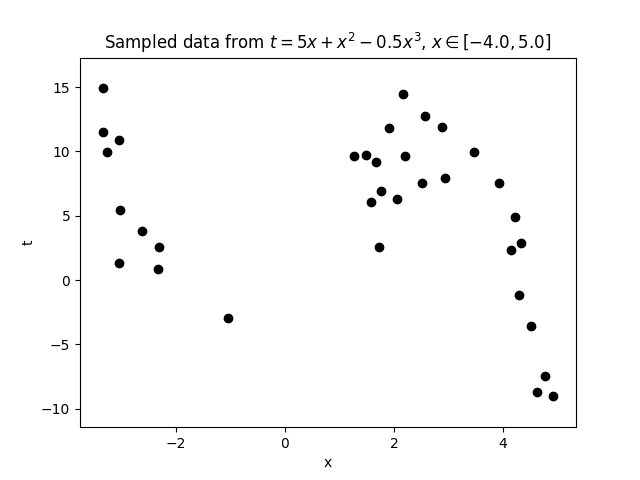
\includegraphics[width=10cm]{figures/ex5_synth_data.png}
%\caption{Your Caption Here.\label{fig:data}}
%\end{center}
%\end{figure}
%
%\begin{figure}[h!]
%\begin{center}
%\subfigure[]{
%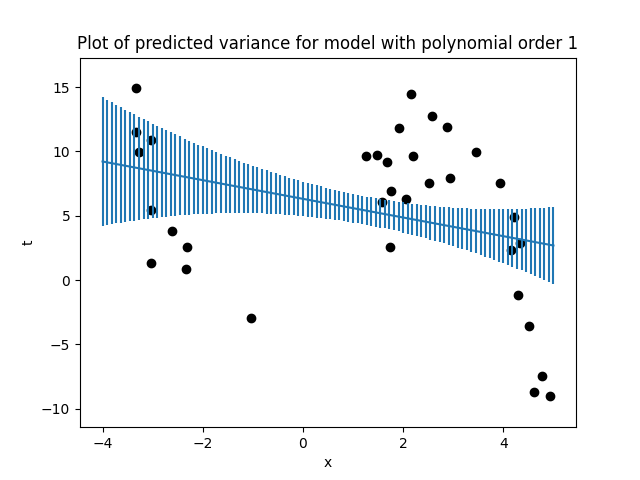
\includegraphics[width=.48\textwidth]{figures/ex5b_fn_errorbars_order-1.png}
%}
%\subfigure[]{
%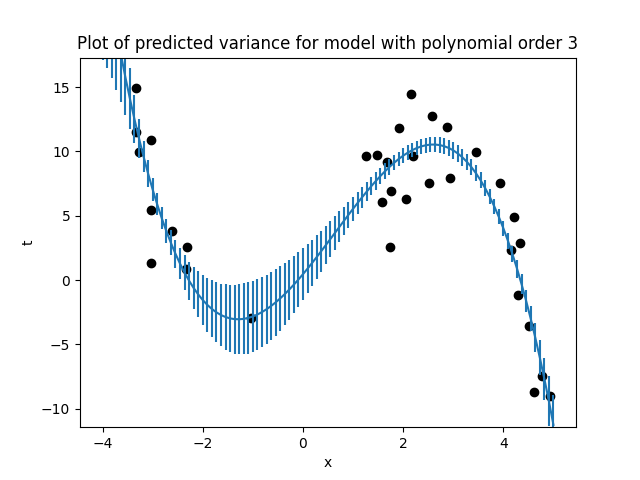
\includegraphics[width=.48\textwidth]{figures/ex5b_fn_errorbars_order-3.png}
%}
%
%\subfigure[]{
%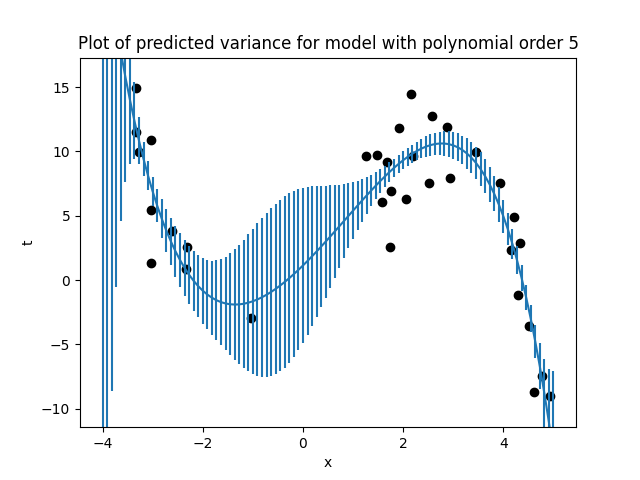
\includegraphics[width=.48\textwidth]{figures/ex5b_fn_errorbars_order-5.png}
%}
%\subfigure[]{
%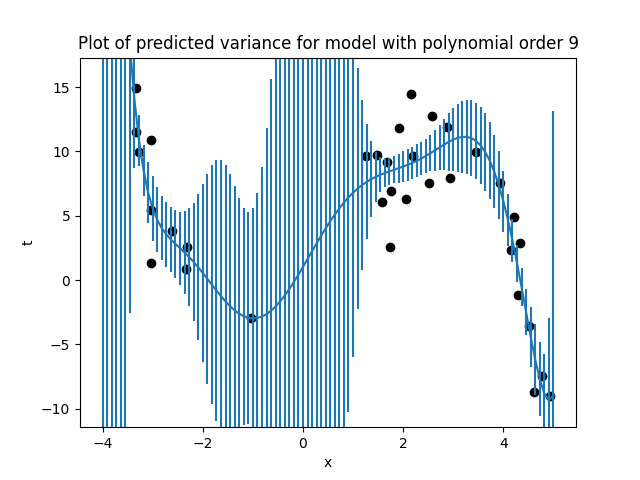
\includegraphics[width=.48\textwidth]{figures/ex5b_fn_errorbars_order-9.png}
%}
%
%\caption{Your Caption Here\label{fig:variance}}
%\end{center}
%\end{figure}
%
%\begin{figure}[h!]
%\begin{center}
%\subfigure[]{
%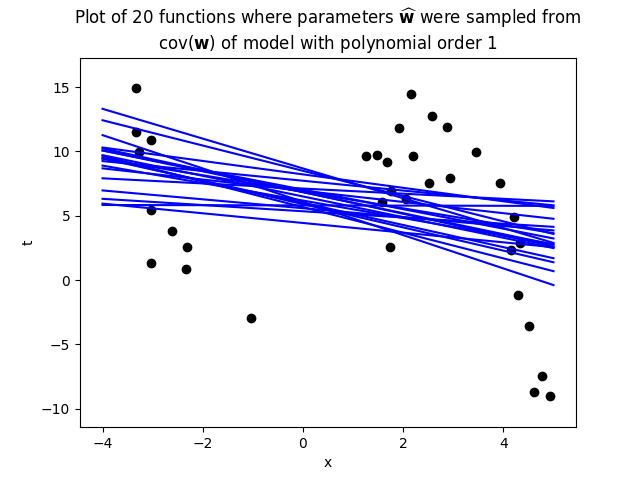
\includegraphics[width=.48\textwidth]{figures/ex5c_sample_fn_order-1.png}
%}
%\subfigure[]{
%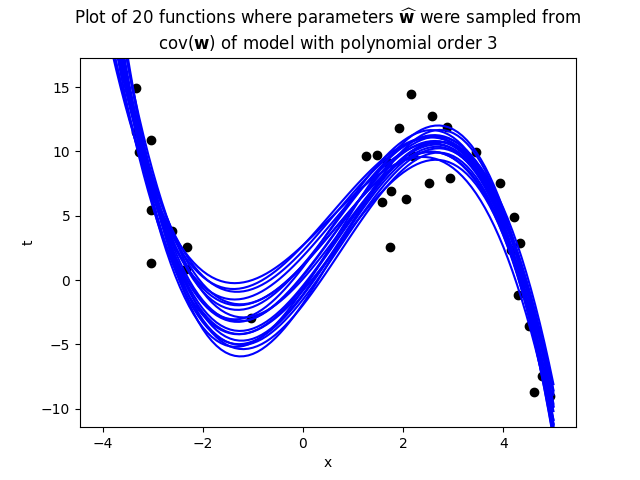
\includegraphics[width=.48\textwidth]{figures/ex5c_sample_fn_order-3.png}
%}
%
%\subfigure[]{
%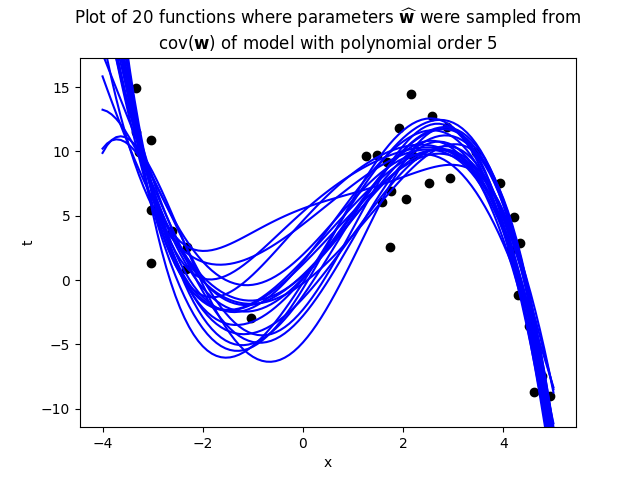
\includegraphics[width=.48\textwidth]{figures/ex5c_sample_fn_order-5.png}
%}
%\subfigure[]{
%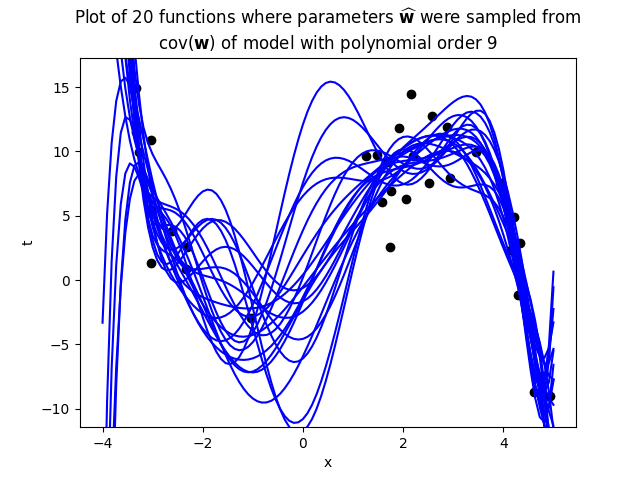
\includegraphics[width=.48\textwidth]{figures/ex5c_sample_fn_order-9.png}
%}
%
%\caption{Your Caption Here.\label{fig:fn-samples}}
%\end{center}
%\end{figure}




%%%     Exercise 6
\item[6.] [5 points]

The code for this exercise is also found in {\tt predictive\_variance.py}, in the function {\tt exercise\_6}.
In this exercise, you will fill in the missing pieces as indicated. Once done, running {\tt exercise\_6} demonstrates how model bias impacts variance, similar to the demonstration in Lecture 9.  % (starting slide 10).  
Once implemented, the script will generate four plots: a separate plot for each of the model polynomial orders 1, 3, 5 and 9. In your written answer, first describe what the code is doing, in your own words. Then, include the four plots with descriptive captions, and describe what happens to the variance in the functions in the plots as the model order is changed.

{\bf Solution.}

%%% For latex users: code to insert figure, and update the caption to describe the figure!
%\begin{figure}[h!]
%\begin{center}
%\subfigure[]{
%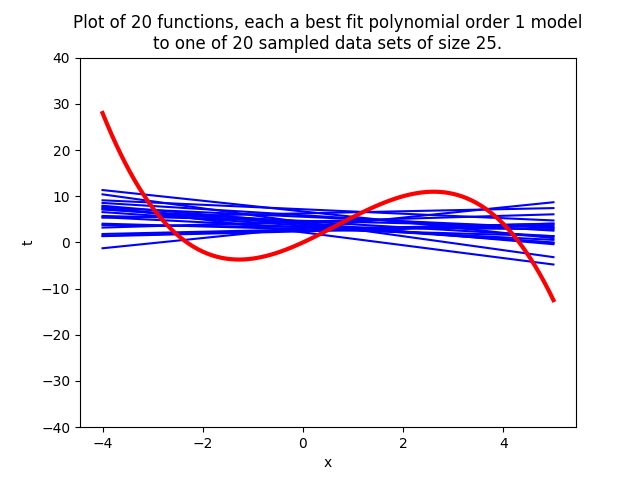
\includegraphics[width=.48\textwidth]{figures/ex6_sample_fn_order-1.png}
%}
%\subfigure[]{
%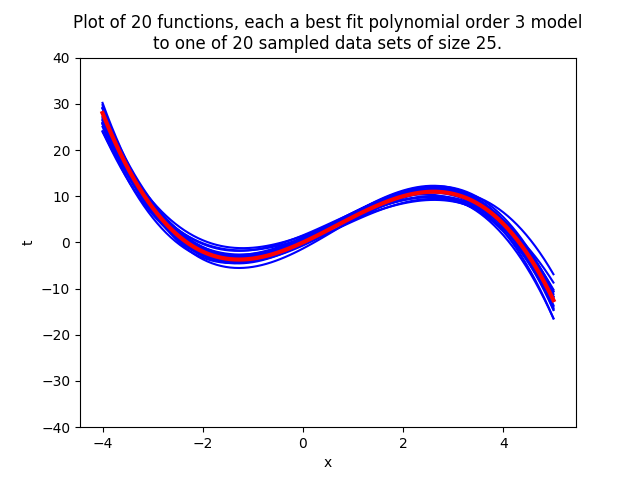
\includegraphics[width=.48\textwidth]{figures/ex6_sample_fn_order-3.png}
%}
%
%\subfigure[]{
%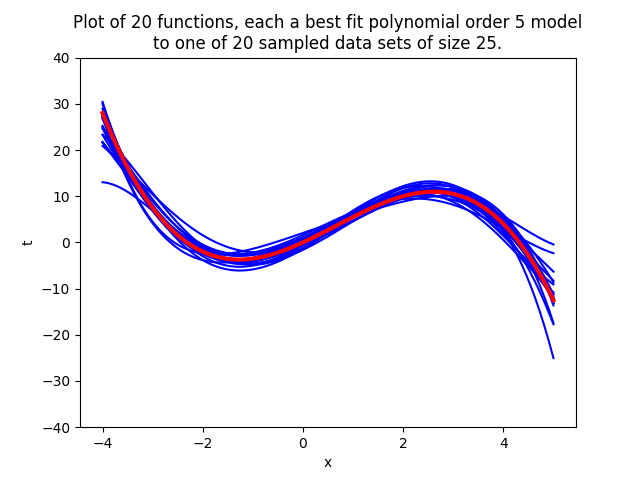
\includegraphics[width=.48\textwidth]{figures/ex6_sample_fn_order-5.png}
%}
%\subfigure[]{
%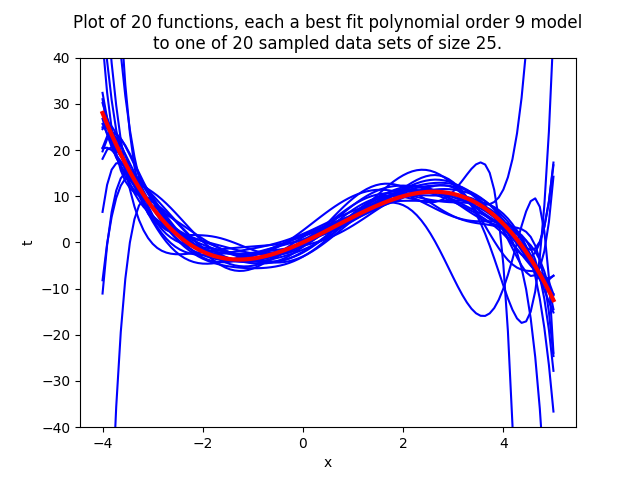
\includegraphics[width=.48\textwidth]{figures/ex6_sample_fn_order-9.png}
%}
%
%\caption{Your Caption Here.\label{fig:fns-to-samples}}
%\end{center}
%\end{figure}
 


%%%     Exercise 7
\item[7.] [4 points; \boldred{Required only for Graduates}]
Adapted from {\bf Exercise 2.13} of FCML:

Derive the Fisher Information Matrix for the parameter of a Bernoulli distribution.

{\bf Solution.}

\end{itemize}

\end{document}